\documentclass[11pt,a4paper]{article}
\usepackage{fontspec}
\setmainfont{cmunrm.otf}[BoldFont=cmunbx.otf,ItalicFont=cmunti.otf,BoldItalicFont=cmunbi.otf]
\setsansfont{cmunss.otf}[BoldFont=cmunsx.otf]
\setmonofont{cmuntt.otf}
\usepackage[russian]{babel}
\usepackage[a4paper,margin=2.3cm]{geometry}
\usepackage{amsmath,amssymb}
\usepackage{graphicx,booktabs,array,tabularx,float}
\usepackage[font=small,labelfont=bf,labelsep=period]{caption}
\usepackage{xcolor,tikz}
\usetikzlibrary{arrows.meta,decorations.markings}
\usepackage[colorlinks,linkcolor=blue!50!black,citecolor=blue!50!black,urlcolor=blue!50!black]{hyperref}
\usepackage{enumitem}
\setlist{itemsep=2pt,topsep=4pt}
\graphicspath{{../figs/}}
\linespread{1.08}

\newcommand{\tb}{t_b}
\newcommand{\he}{h/e^2}
\newcommand{\Rxy}{R_{xy}}
\newcommand{\Rxx}{R_{xx}}
\newcommand{\lB}{l_B}
\newcommand{\EF}{E_F}
\newcommand{\hw}{\hbar\omega_c}

\definecolor{chiral}{HTML}{0b0b0b}
\definecolor{counter}{HTML}{eb6834}
\definecolor{pocket}{HTML}{2a78d6}

\title{Встречные краевые каналы в «кармане»\\ удерживающего потенциала
и холловский отклик\\[4pt]
\large численное исследование}
\author{Рабочая заметка}
\date{28 сентября 2026}

\begin{document}
\maketitle

\begin{abstract}
\noindent
Мы численно (Kwant, модель сильной связи) исследуем шеститерминальный
холловский мостик, у края которого удерживающий потенциал образует яму
(«карман»). В кармане следующий уровень Ландау пересекает уровень Ферми
дважды, и у края появляется пара каналов, один из которых бежит против
киральности. Всё, что происходит с такой парой между двумя соседними
контактами, сводится к одному числу~--- вероятности обратного прохождения
$\tb$; через него явно выражаются холловское и продольное сопротивления.
Квантование нарушается, когда встречный канал доходит до контакта
($\tb\neq0$). Обратное рассеяние внутри пары, наоборот, его восстанавливает.
С потенциалом изображения из работы~\cite{andolina} картина та же.
Двухтерминальный кондактанс, на котором основаны выводы~\cite{andolina},
равен $\nu+\tb$ и потому целый и при $\tb=0$, и при $\tb=1$; он не замечает
как раз того режима, где холловский мостик даёт наибольшее отклонение.
В конце перечислены признаки механизма, проверяемые в четырёхтерминальной
геометрии.
\end{abstract}

\tableofcontents

%======================================================================
\section{Постановка вопроса}

В экспериментах с двумерным электронным газом GaAs внутри металлического
кольцевого резонатора наблюдалось искажение плато квантового эффекта Холла
(КЭХ)~\cite{appugliese}. Первоначально его объясняли вакуумными флуктуациями
поля резонатора. В работе~\cite{andolina} предложено электростатическое
объяснение: изображение электрона в металле резонатора, стоящем рядом с
краем мезы, притягивает электрон к краю. Вместе с крутым удерживающим
потенциалом это даёт яму у края, в которой возникают встречные
(некиральные) краевые каналы. Авторы~\cite{andolina} считают только
двухтерминальный кондактанс $G(\EF)$. В комментарии~\cite{ciuti} возражают,
что (i)~самосогласованная электростатика GaAs-мезы кармана не даёт и
(ii)~эксперимент измеряет $\Rxx$ и $\Rxy$ в холловском мостике, а не
двухтерминальный кондактанс.

Здесь мы не спорим о том, есть ли карман (пункт~(i)): карман задан руками.
Нас интересует, \emph{что он сделает с холловским откликом, если он есть}:
\begin{enumerate}
\item портит ли встречный канал на одном краю $\Rxy$ и $\Rxx$
      шеститерминального мостика;
\item при каких условиях (перекрытие партнёров, беспорядок, геометрия
      контактов);
\item как это соотносится с выводами~\cite{andolina}, полученными из
      двухтерминального кондактанса.
\end{enumerate}
Резонатор как динамическая система не рассматривается.

%======================================================================
\section{Модель}

\subsection{Гамильтониан и единицы}
Квадратная решётка с постоянной $a=1$ и прыжком $t=1$:
\begin{equation}
H=\sum_i\bigl(4t+V_i\bigr)c_i^\dagger c_i-t\sum_{\langle ij\rangle}
e^{i\theta_{ij}}c_i^\dagger c_j,
\end{equation}
фазы Пайерлса $\theta_{ij}$ соответствуют потоку $\varphi$ квантов $h/e$ на
плакетку. В континуальном пределе
$\hw\simeq4\pi\varphi\,t$, $\lB=a/\sqrt{2\pi\varphi}$.
Энергия Ферми по умолчанию фиксирована, $\EF=0.4\,t$; поле развёртывается в
диапазоне $\varphi=0.008\ldots0.06$ (плато $\nu=4\ldots1$,
$\lB\approx1.6\ldots4.5\,a$). Калибровка поля проверена по расстоянию между
уровнями Ландау в ленте в калибровке Ландау и по положению плато.

\subsection{Геометрия}
Мостик $300\times80$ с четырьмя зондами шириной $56$ (много больше ширины
кармана и $\lB$) и шестью идеальными омическими контактами~---
полубесконечными подводами в том же поле и с тем же профилем края
(рис.~\ref{fig:scheme}). Ток пропускается $0\to3$, зонды 1, 2, 4, 5
плавающие. При нашем знаке поля электроны обходят периметр как
$0\to5\to4\to3\to2\to1\to0$.

\begin{figure}[ht]
\centering
\begin{tikzpicture}[x=1.45cm,y=1.45cm,
  chir/.style={chiral,thick,decoration={markings,mark=at position 0.55 with {\arrow{Stealth[length=2.2mm]}}},postaction=decorate},
  ctr/.style={counter,thick,dashed,decoration={markings,mark=at position 0.55 with {\arrow{Stealth[length=2.2mm]}}},postaction=decorate}]
  % sample
  \fill[black!5] (-0.6,0) -- (1.4,0) -- (1.4,-0.9) -- (3.2,-0.9) -- (3.2,0) -- (4.8,0) -- (4.8,-0.9)
    -- (6.6,-0.9) -- (6.6,0) -- (8.6,0) -- (8.6,2) -- (6.6,2) -- (6.6,2.9) -- (4.8,2.9) -- (4.8,2)
    -- (3.2,2) -- (3.2,2.9) -- (1.4,2.9) -- (1.4,2) -- (-0.6,2) -- cycle;
  % pocket band along the bottom edge
  \fill[pocket!15] (-0.6,0) rectangle (8.6,0.32);
  \fill[pocket!15] (1.4,-0.9) rectangle (1.72,0); \fill[pocket!15] (2.88,-0.9) rectangle (3.2,0);
  \fill[pocket!15] (4.8,-0.9) rectangle (5.12,0); \fill[pocket!15] (6.28,-0.9) rectangle (6.6,0);
  % outline
  \draw[thick] (-0.6,0) -- (1.4,0) -- (1.4,-0.9) (3.2,-0.9) -- (3.2,0) -- (4.8,0) -- (4.8,-0.9)
               (6.6,-0.9) -- (6.6,0) -- (8.6,0);
  \draw[thick] (-0.6,2) -- (1.4,2) -- (1.4,2.9) (3.2,2.9) -- (3.2,2) -- (4.8,2) -- (4.8,2.9)
               (6.6,2.9) -- (6.6,2) -- (8.6,2);
  % contacts
  \foreach \x/\y/\n in {-0.9/1/0, 8.9/1/3, 2.3/-1.15/1, 5.7/-1.15/2, 5.7/3.15/4, 2.3/3.15/5}
    \node[font=\bfseries] at (\x,\y) {\n};
  % chiral channels
  \draw[chir] (-0.6,1.85) -- (1.25,1.85);
  \draw[chir] (1.25,1.85) -- (1.25,2.9);
  \draw[chir] (3.35,2.9) -- (3.35,1.85) -- (4.65,1.85);
  \draw[chir] (4.65,1.85) -- (4.65,2.9);
  \draw[chir] (6.75,2.9) -- (6.75,1.85) -- (8.6,1.85);
  \draw[chir] (8.6,0.45) -- (6.75,0.45) -- (6.75,-0.9);
  \draw[chir] (4.65,-0.9) -- (4.65,0.45) -- (3.35,0.45);
  \draw[chir] (3.35,0.45) -- (3.35,-0.9);
  \draw[chir] (1.25,-0.9) -- (1.25,0.45) -- (-0.6,0.45);
  % counter-propagating channel in the pocket
  \draw[ctr] (-0.6,0.22) -- (1.52,0.22) -- (1.52,-0.9);
  \draw[ctr] (3.08,-0.9) -- (3.08,0.22) -- (4.92,0.22) -- (4.92,-0.9);
  \draw[ctr] (6.48,-0.9) -- (6.48,0.22) -- (8.6,0.22);
  \node[counter,font=\small] at (4,-0.35) {$\tb$};
  \node[font=\small,align=center] at (4,1.1) {объём: $\nu$ заполненных уровней};
  \node[pocket!70!black,font=\small] at (7.6,-0.35) {карман};
\end{tikzpicture}
\caption{Схема мостика. Чёрные стрелки~--- $\nu$ киральных каналов на каждом
краю (показан один). Голубая полоса~--- карман у нижнего края (включая нижние
зонды и нижние половины подводов 0 и~3). Оранжевый пунктир~--- встречный
канал на внутренней границе кармана; его сонаправленный партнёр на внешней
границе не показан. $\tb$~--- вероятность того, что электрон, выпущенный
контактом ниже по течению, дойдёт против киральности до контакта выше по
течению.}
\label{fig:scheme}
\end{figure}

\subsection{Профиль края}
Потенциал зависит от расстояния $d$ до границы образца. Стенка гладкая:
\[
V_\text{wall}(d)=V_w\Bigl(\frac{d_0-d}{d_0}\Bigr)^2\theta(d_0-d),\qquad
V_w=1.5\,t,\ d_0=6\,a .
\]
Рассмотрены два вида кармана.
\begin{itemize}
\item \textbf{Прямоугольный карман} (разделы~\ref{sec:rect}):
  $V(d)=V_\text{wall}(d)-V_\text{dip}\,w(d;d_\text{in},d_\text{out})$, где
  $w$~--- сглаженное окно ($\tanh$ с шириной фронта $a$), $d_\text{in}=6$.
  \emph{Широкий} карман: $V_\text{dip}=0.3\,t$, ширина $14\,a$, пара
  разнесена на $\approx5.8\,\lB$ (при $\nu=1$, $\varphi=0.028$), перекрытие
  $<0.01$. \emph{Узкий}: $V_\text{dip}=0.35\,t$, ширина $4\,a$, разнесение
  $\approx1.6\,\lB$, перекрытие $\approx0.57$.
\item \textbf{Потенциал изображения} (раздел~\ref{sec:image}), форма
  из~\cite{andolina}: металл параллелен краю на расстоянии $d_\text{edge}$,
  \begin{equation}\label{eq:img}
  V(d)=V_\text{wall}(d)-E_\text{img}\Bigl[\frac1{d+d_\text{edge}}-
  \frac1{d_c+d_\text{edge}}\Bigr]\theta(d_c-d),
  \end{equation}
  $d_c=40\,a$ (середина мостика), так что объём и противоположный край не
  затронуты.
\end{itemize}
Перекрытие партнёров определяем как $O=\sum_y|\psi_1(y)||\psi_2(y)|$
($1$~--- совпадающие, $0$~--- непересекающиеся волновые функции моды в
бесконечной ленте с тем же профилем).

Варианты расположения кармана: только нижний край; оба края; \emph{локальный}
карман на нижнем крае между зондами 1 и 2, не касающийся ни одного контакта.
Беспорядок Андерсона $U=1\,t$ (равномерно в $[-U/2,U/2]$) во всей
рассеивающей области; «чистые» расчёты~--- с $U=0$.

\subsection{Наблюдаемые}
Из матрицы рассеяния Kwant~\cite{kwant} находим матрицу кондактансов
$G_{ij}$, задаём ток $I$ из контакта 0 в контакт 3 (заземлён) и находим
потенциалы плавающих зондов. Далее (все сопротивления в $\he$):
\[
\Rxy^{(1\text{--}5)}=\frac{V_5-V_1}{I},\quad
\Rxy^{(2\text{--}4)}=\frac{V_4-V_2}{I},\quad
\Rxx^{\text{низ}}=\frac{V_1-V_2}{I},\quad
\Rxx^{\text{верх}}=\frac{V_5-V_4}{I},\quad
R_\text{2t}=\frac{V_0-V_3}{I}.
\]
Для сравнения с~\cite{andolina} отдельно считается двухтерминальный
кондактанс $G_\text{2t}$ простого бруска $300\times80$ без зондов с тем же
профилем края.

%======================================================================
\section{Откуда берётся встречный канал}

Для плавного на масштабе $\lB$ потенциала уровни Ландау повторяют его ход,
$E_n(y)\approx\hw(n+\tfrac12)+V(y)$, а групповая скорость вдоль края
пропорциональна $\partial_yV$. Пусть в объёме $\EF$ лежит между уровнями $n$
и $n+1$. Если в кармане уровень $n+1$ опускается ниже $\EF$, он пересекает
$\EF$ дважды. Внешнее пересечение (со стороны стенки) даёт канал,
сонаправленный с киральными; внутреннее, где $\partial_yV$ другого знака,~---
\emph{встречный} канал. Это происходит на низкополевой стороне каждого плато,
пока $(n+\tfrac32)\hw-V_\text{dip,eff}<\EF$ (рис.~\ref{fig:edge}). Узкий
карман даёт пару на расстоянии порядка $\lB$, широкий~--- разнесённую.

\begin{figure}[ht]
\centering
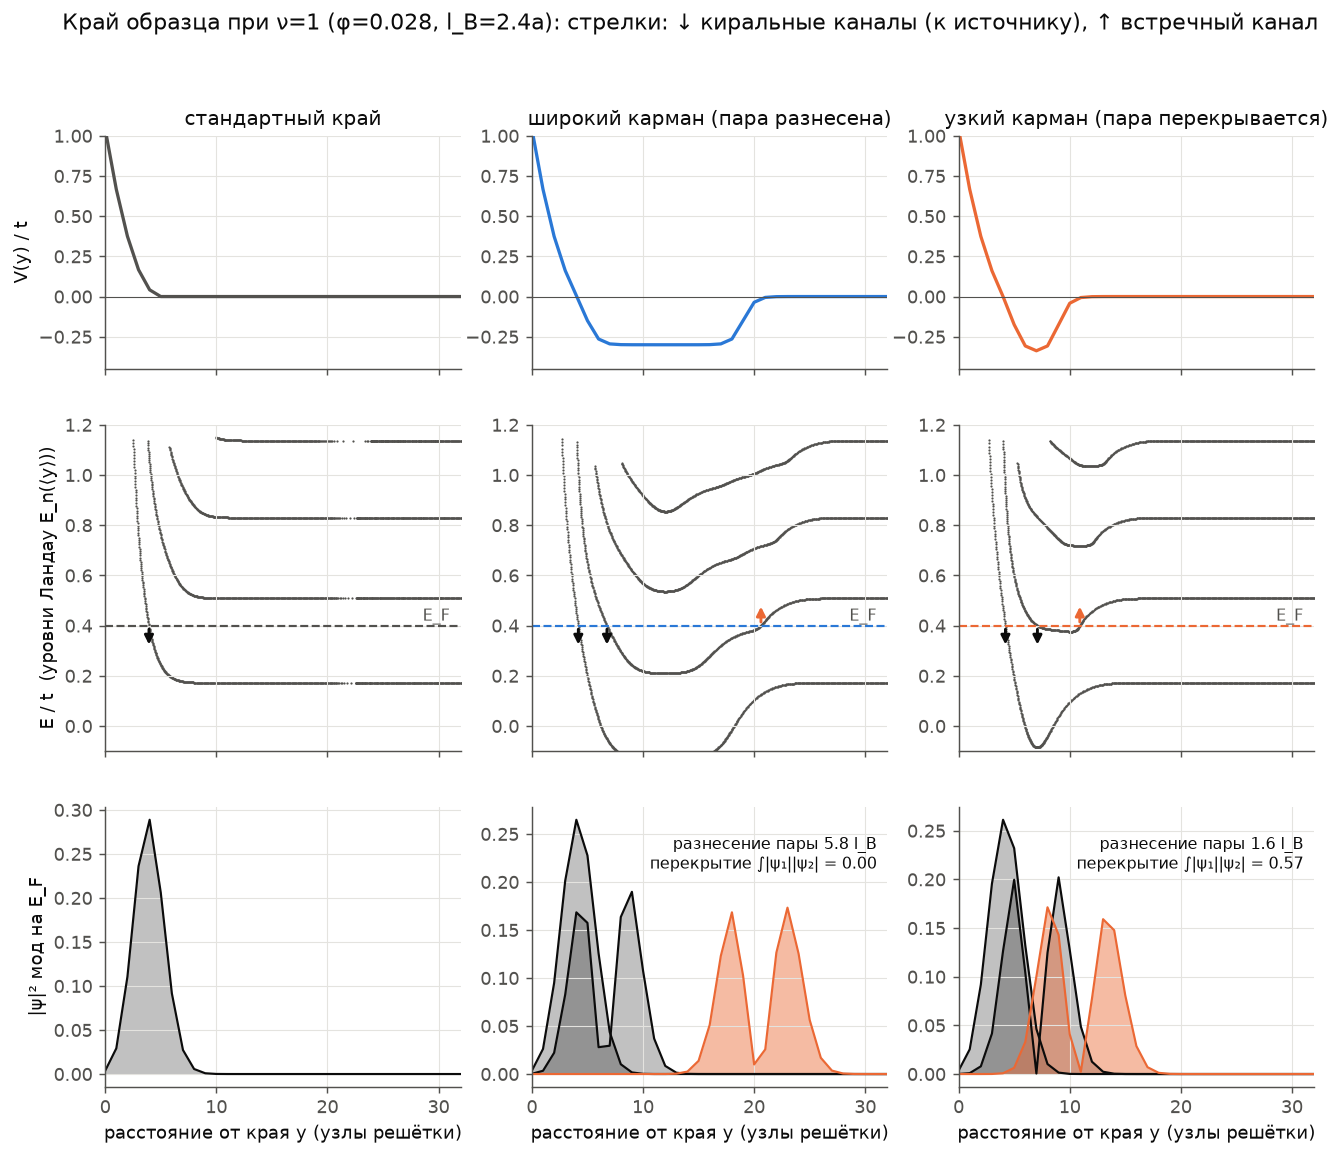
\includegraphics[width=\textwidth]{fig1_edge_structure.png}
\caption{Край при $\nu=1$ ($\varphi=0.028$). Сверху вниз: профиль
потенциала; собственные энергии ленты в зависимости от положения состояния
$\langle y\rangle$ (изогнутые уровни Ландау) со стрелками мод на $\EF$
(чёрные~--- киральные, оранжевые~--- встречные); профили мод на $\EF$.
Слева направо: стандартный край, широкий и узкий карманы.}
\label{fig:edge}
\end{figure}

%======================================================================
\section{Общее утверждение: один параметр $\tb$}\label{sec:lb}

\subsection{Сегмент края}
Рассмотрим участок края между соседними контактами $a$ (выше по течению) и
$b$ (ниже). На нём $\nu$ киральных каналов и пара (сонаправленный +
встречный). Из $a$ в сегмент уходят $\nu+1$ каналов, в $a$ из сегмента
приходит один (встречный); из $b$ в сегмент уходит один канал, в $b$
приходят $\nu+1$. Если ток не уходит через объём в другие контакты,
унитарность матрицы рассеяния сегмента даёт
\[
T_{a\leftarrow b}+R_{b}=1,\qquad T_{b\leftarrow a}+R_{b}=\nu+1
\quad\Longrightarrow\quad
T_{b\leftarrow a}-T_{a\leftarrow b}=\nu .
\]
Каким бы ни было рассеяние внутри сегмента (упругое обратное рассеяние,
перемешивание каналов, частичная эквилибрация), сегмент полностью описывается
одним числом~--- \emph{вероятностью обратного прохождения}
$\tb\equiv T_{a\leftarrow b}\in[0,1]$. $\tb=0$~--- идеальный край КЭХ,
$\tb=1$~--- баллистический встречный канал.

\subsection{Формулы для мостика}
Для кармана на нижнем крае с одинаковым $\tb$ на всех трёх сегментах
нижнего края формулы Ландауэра--Бюттикера~\cite{buttiker} решаются
символьно (табл.~\ref{tab:lb}).

\begin{table}[ht]
\centering
\caption{Сопротивления мостика с карманом на нижнем крае (в $\he$).}
\label{tab:lb}
\begin{tabular}{lcc}
\toprule
величина & формула & $\nu=1,\ \tb=1$\\
\midrule
$\Rxy^{(1\text{--}5)}$ & $1/(\nu+\tb)$ & $1/2$\\
$\Rxy^{(2\text{--}4)}$ & $(\nu+2\tb)/(\nu+\tb)^2$ & $3/4$\\
$\Rxx^\text{низ}$ & $\tb/(\nu+\tb)^2$ & $1/4$\\
$\Rxx^\text{верх}$ & $0$ & $0$\\
$R_\text{2t}$ (с плавающими зондами) & $(\nu^2+3\nu\tb+3\tb^2)/(\nu+\tb)^3$ & $7/8$\\
\bottomrule
\end{tabular}
\end{table}

Для простого двухтерминального бруска, у которого подводы несут тот же край,
\begin{equation}\label{eq:g2t}
G_\text{2t}=\nu+\tb^{\text{(вся длина)}}\quad[e^2/h],
\end{equation}
где $\tb$ берётся по всей длине края от стока до истока.

\subsection{Следствия}
\begin{itemize}
\item \textbf{Квантование портит не обратное рассеяние, а его отсутствие.}
  Баллистический встречный канал ($\tb=1$) переносит потенциал контакта,
  стоящего ниже по течению, к контакту выше по течению. Это сдвигает
  $\Rxy$ и даёт $\Rxx\neq0$ без всякой диссипации в объёме; объёмная
  $\sigma_{xy}=\nu e^2/h$ остаётся топологической.
\item \textbf{Обратное рассеяние внутри пары лечит.} Если партнёры
  перекрываются и беспорядок рассеивает электроны назад, встречный канал
  локализуется вдоль края, $\tb\sim e^{-L/\xi}\to0$, и квантование
  восстанавливается.
\item \textbf{Нужен контакт.} Если карман локальный и не касается
  омических контактов, пара образует замкнутую петлю, $\tb\equiv0$, и
  эффекта в постоянном токе нет.
\item Край без кармана остаётся идеальным ($\Rxx^\text{верх}=0$), а разность
  двух холловских напряжений в точности равна $\Rxx$ дефектного края.
\end{itemize}

%======================================================================
\section{Прямоугольный карман}\label{sec:rect}

\subsection{Карман на одном (нижнем) крае}
На рис.~\ref{fig:sweeps} серые кривые~--- стандартный образец: плато
$\Rxy=h/\nu e^2$ и $\Rxx=0$, между плато~--- типичные для малого когерентного
образца мезоскопические флуктуации. Кривые усреднены по трём реализациям
беспорядка.

\begin{figure}[ht]
\centering
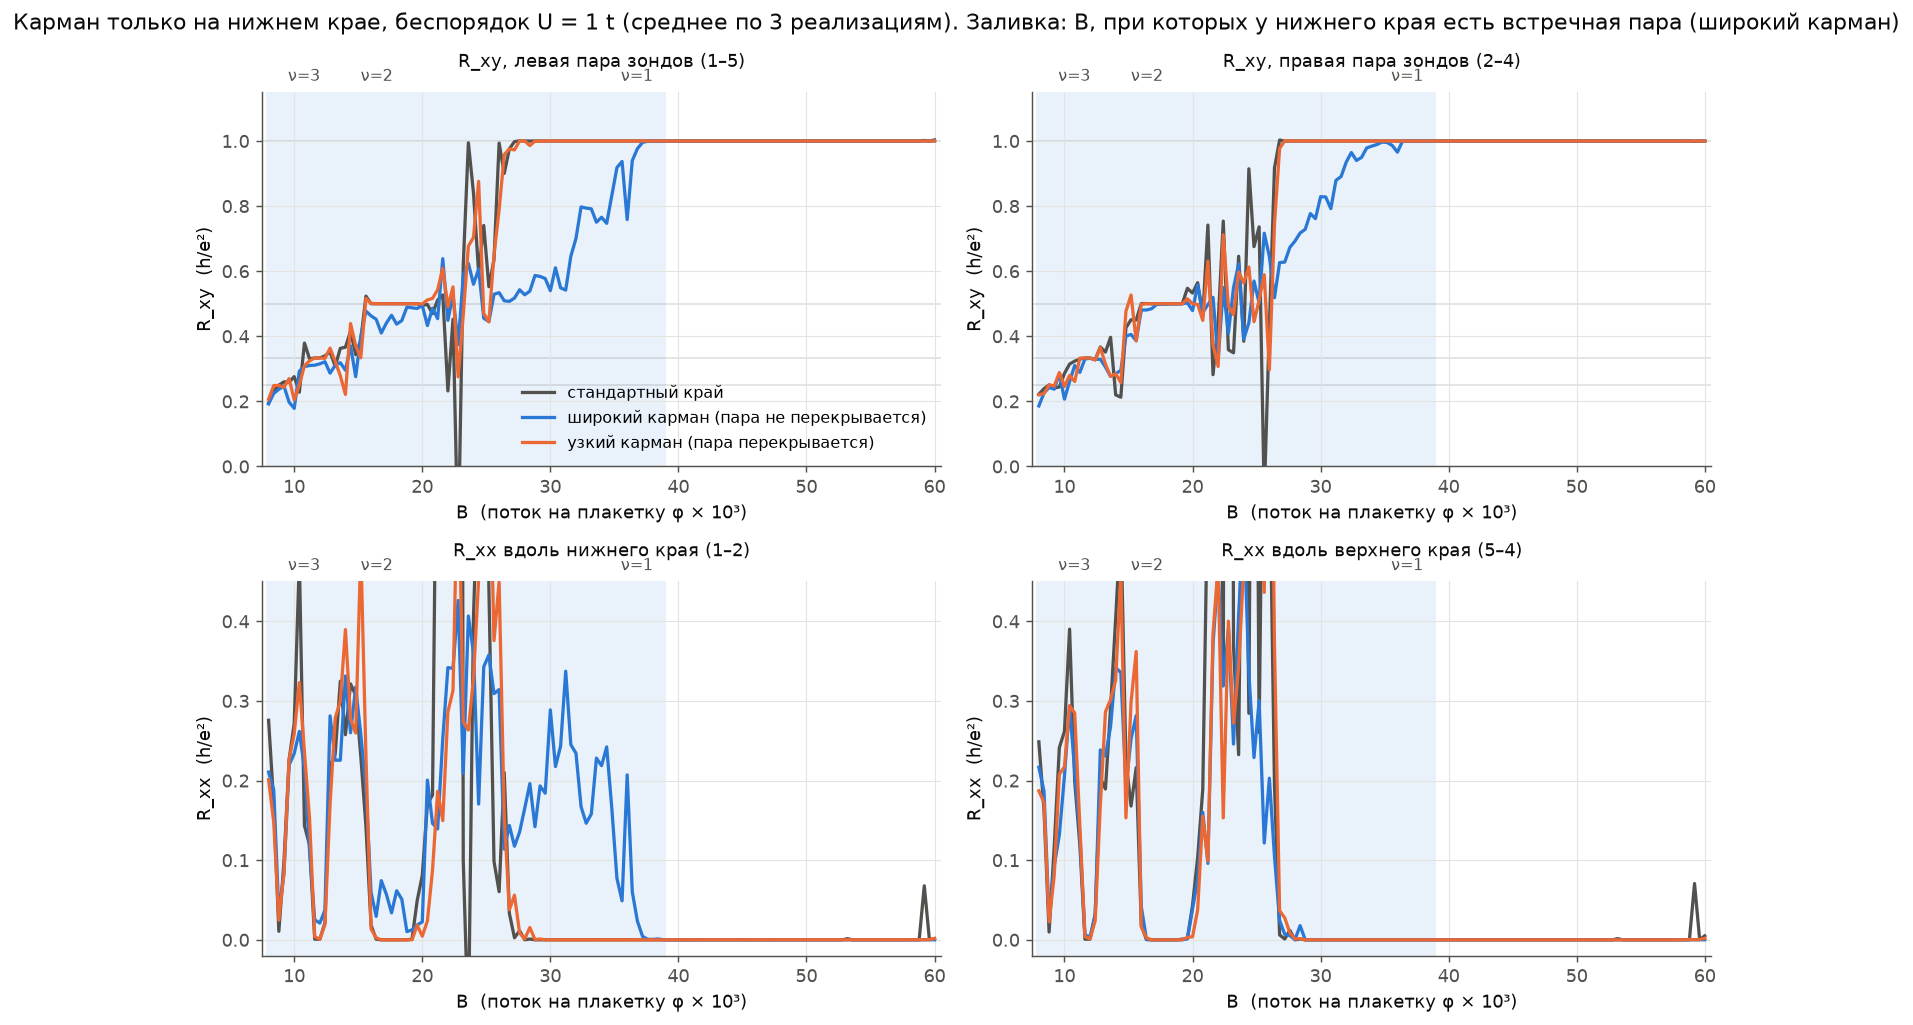
\includegraphics[width=\textwidth]{fig2_sweeps_bottom_pocket.png}
\caption{Развёртка по полю при $\EF=0.4\,t$, $U=1\,t$, среднее по трём
реализациям. Заливка~--- поля, при которых у нижнего края есть встречная пара
(широкий карман).}
\label{fig:sweeps}
\end{figure}

\begin{itemize}
\item \textbf{Широкий карман} (пара разнесена на 4--6~$\lB$): на
  низкополевой части плато $\nu=1$ ($\varphi\approx0.027$--$0.038$)
  $\Rxy^{(1\text{--}5)}$ опускается до $\approx0.53$, а
  $\Rxy^{(2\text{--}4)}$~--- до $\approx0.67$. $\Rxx^\text{низ}$ доходит до
  $\approx0.34$, а $\Rxx^\text{верх}=0$ с точностью $10^{-4}$ при
  $\varphi>0.03$. Слабее то же видно на плато $\nu=2$. При $\varphi>0.039$
  пары нет, и кривые совпадают с эталоном.
\item \textbf{Узкий карман} (разнесение $\approx1.6\,\lB$, перекрытие
  $\approx0.6$): пара существует при $\varphi\approx0.022$--$0.029$, частично
  внутри перехода $2\to1$. На участке плато $\varphi\approx0.0275$--$0.029$
  беспорядок возвращает $\Rxy$ к $\he$ с точностью $\approx0.01$, тогда как
  без беспорядка там же $\Rxy^{(1\text{--}5)}=0.5$ (рис.~\ref{fig:clean}).
\end{itemize}

\subsection{Без беспорядка и с беспорядком}
Без беспорядка встречный канал баллистический, $\tb=1$, и Kwant
\emph{точно} воспроизводит табл.~\ref{tab:lb}:
$\Rxy^{(1\text{--}5)}=1/(\nu+1)$ ($0.5$; $0.333$; $0.25$ при $\nu=1,2,3$),
$\Rxy^{(2\text{--}4)}=(\nu+2)/(\nu+1)^2$ ($0.75$; $0.444$; $0.3125$),
$\Rxx^\text{низ}=1/(\nu+1)^2$ ($0.25$; $0.111$; $0.0625$)~--- на всём
интервале полей, где есть пара. Это верно \emph{и для узкого кармана}: сама
по себе встречная пара, даже перекрытая, без рассеивателей даёт максимальное
отклонение. Включение беспорядка в узком кармане возвращает точное
квантование (рис.~\ref{fig:clean}).

\begin{figure}[ht]
\centering
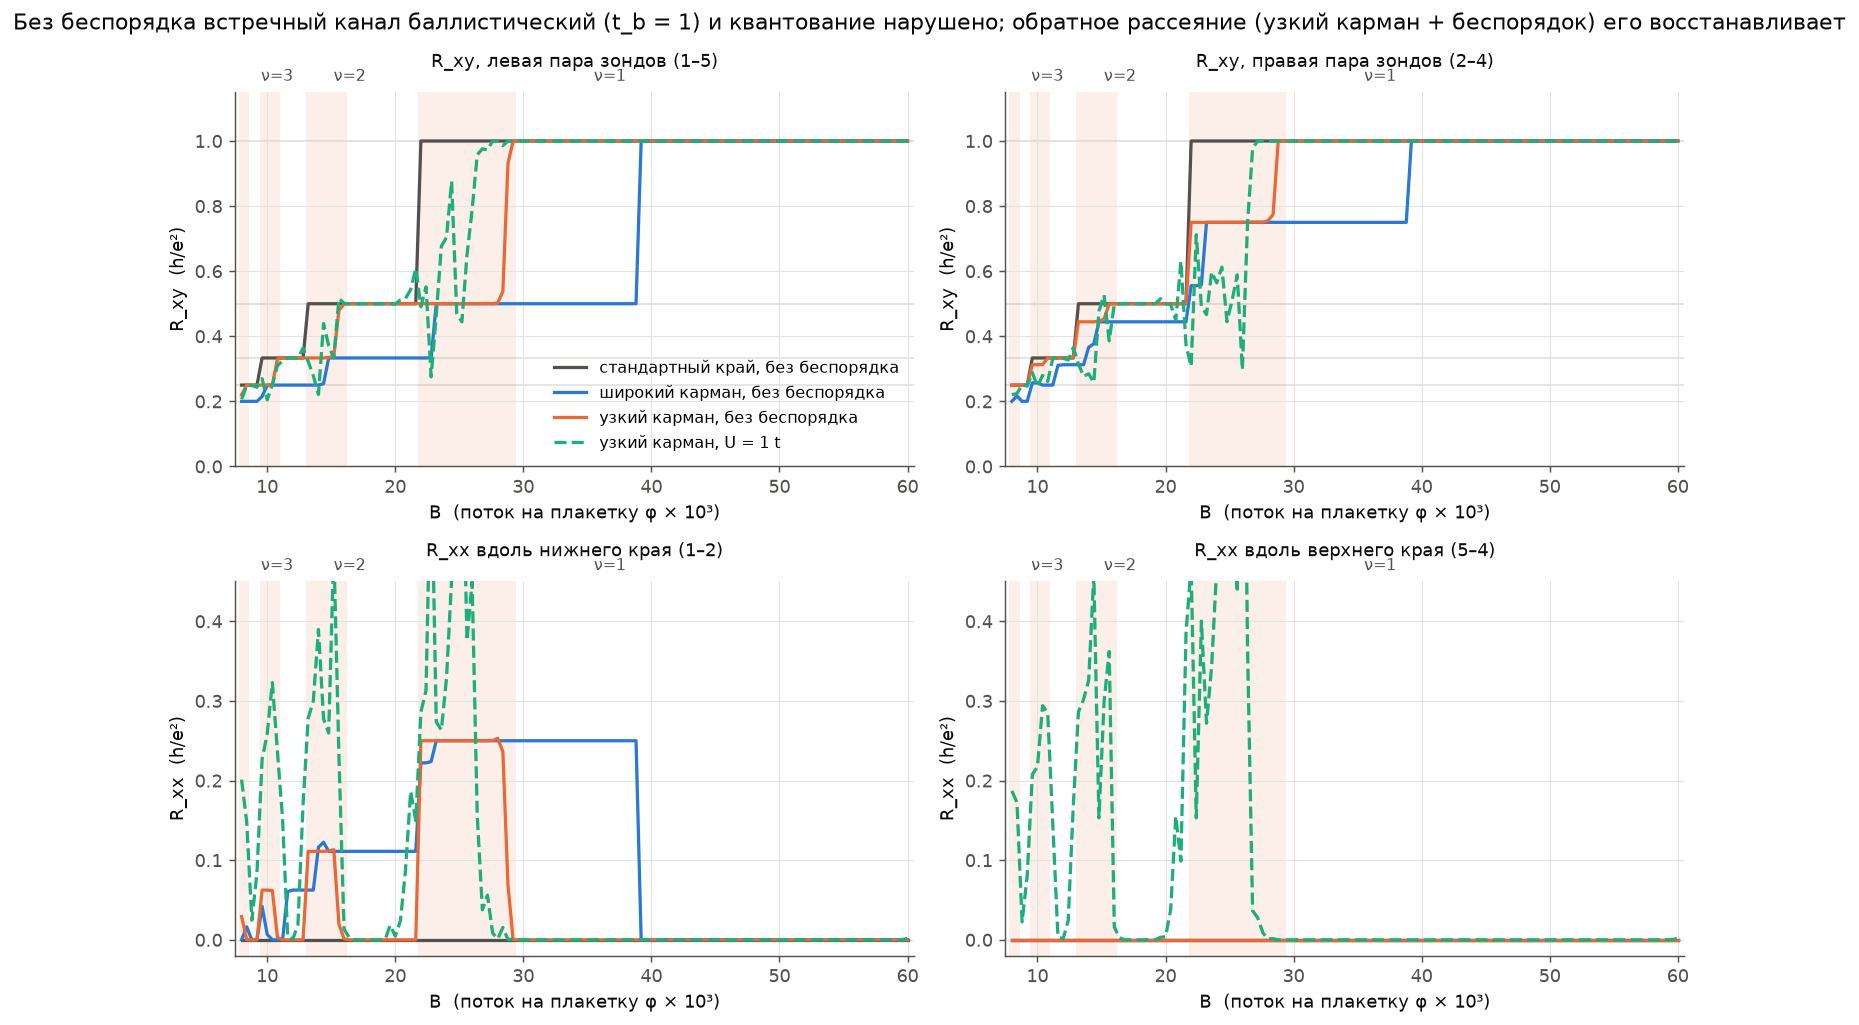
\includegraphics[width=\textwidth]{fig3_clean_vs_disorder.png}
\caption{Без беспорядка ($\tb=1$) квантование нарушено по формулам
табл.~\ref{tab:lb}; обратное рассеяние (узкий карман + беспорядок, зелёный
пунктир) его восстанавливает.}
\label{fig:clean}
\end{figure}

На рис.~\ref{fig:tb} слева~--- $\tb$ между зондами 1 и 2, извлечённое прямо из
матрицы рассеяния; справа~--- формулы табл.~\ref{tab:lb} и точки Kwant на
плато. В широком кармане с беспорядком часть встречного потока проходит мимо
зонда (например, $0\to2$ в обход зонда 1 с вероятностью $\approx0.1$),
поэтому формула с одним $\tb$ там приближённая. Все кривые на рисунках
посчитаны по полной матрице прохождений, а не по этой формуле.

\begin{figure}[ht]
\centering
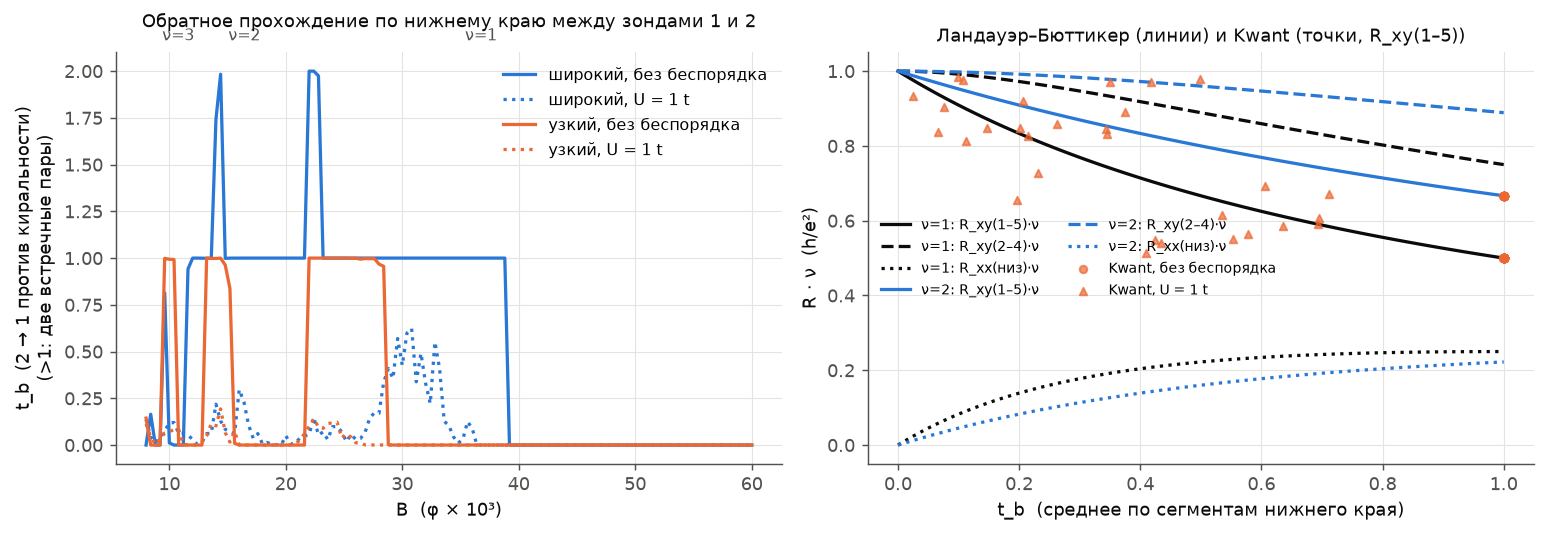
\includegraphics[width=\textwidth]{fig5_tb_and_LB.png}
\caption{Слева: обратное прохождение $\tb$ по нижнему краю между зондами 1
и~2. Справа: формулы Ландауэра--Бюттикера (линии) и Kwant (точки,
$\Rxy^{(1\text{--}5)}$).}
\label{fig:tb}
\end{figure}

\subsection{Перекрываются ли партнёры: ширина кармана}
При фиксированном поле ($\nu=1$, $\varphi=0.028$), глубине кармана
$0.35\,t$ и $U=1\,t$ (три реализации) меняется только ширина кармана, т.\,е.
расстояние между встречными каналами (рис.~\ref{fig:width},
табл.~\ref{tab:width}). Пока партнёры перекрываются, беспорядок рассеивает
электроны внутри пары назад, встречный канал локализуется на длине, меньшей
расстояния между контактами, и отклик квантован. Когда партнёры разнесены,
обратного рассеяния нет, встречный канал доходит до контакта, и квантование
нарушается.

\begin{table}[ht]
\centering
\caption{Зависимость от разнесения пары ($\nu=1$, среднее по трём реализациям).}
\label{tab:width}
\begin{tabular}{lcccc}
\toprule
разнесение пары & $\le2.3\,\lB$ & $2.7\,\lB$ & $3.5\,\lB$ & $\ge4.3\,\lB$\\
\midrule
перекрытие $O$ & 0.9--0.5 & 0.43 & 0.20 & $\le0.06$\\
$\tb$ (сегмент 1--2) & $\approx0$--0.01 & 0.03 & 0.18 & 0.2--0.4\\
$\Rxy^{(1\text{--}5)}$, $\he$ & 0.97--1.00 & 0.94 & 0.75 & 0.53--0.58\\
$\Rxx^\text{низ}$, $\he$ & $\le0.03$ & 0.06 & 0.19 & 0.15--0.27\\
\bottomrule
\end{tabular}
\end{table}

\begin{figure}[ht]
\centering
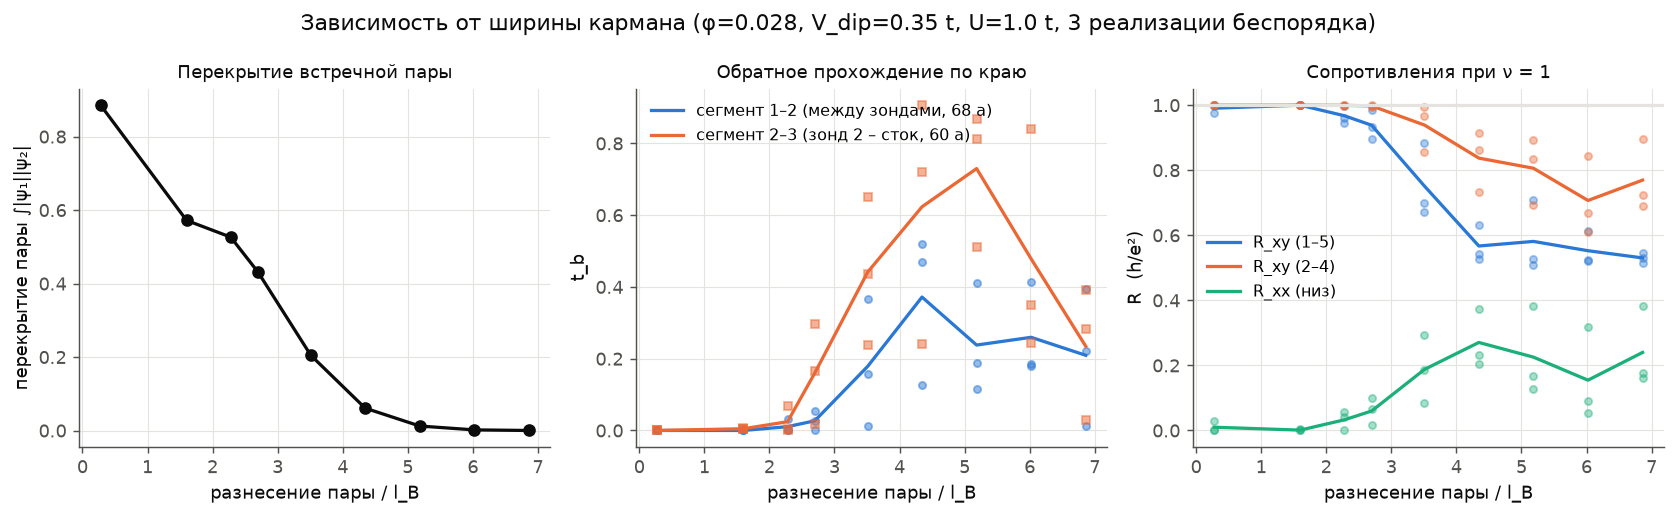
\includegraphics[width=\textwidth]{fig6_width_sweep.png}
\caption{Зависимость от ширины кармана: перекрытие пары, обратное
прохождение по двум сегментам нижнего края и сопротивления при $\nu=1$.
Точки~--- отдельные реализации беспорядка, линии~--- средние.}
\label{fig:width}
\end{figure}

\subsection{Карманы на обоих краях и локальный карман}
\begin{itemize}
\item Широкие карманы на обоих краях: отклонения складываются. При
  баллистической паре формулы Ландауэра--Бюттикера дают $\Rxy=1/3$,
  $\Rxx=2/9$ при $\nu=1$; Kwant с беспорядком~--- $\Rxy\approx0.33$--$0.4$.
\item Узкие карманы на обоих краях с беспорядком: квантование сохраняется,
  $|\Rxy-\he|\le3\cdot10^{-3}$ на плато $\nu=1$ (одна реализация).
\item Широкий карман только на участке нижнего края между зондами 1 и 2, не
  доходящий ни до одного контакта: пара замкнута в петлю, $\tb\equiv0$, и
  кривые совпадают с эталоном~--- хотя обратного рассеяния внутри петли нет.
\end{itemize}

\begin{figure}[ht]
\centering
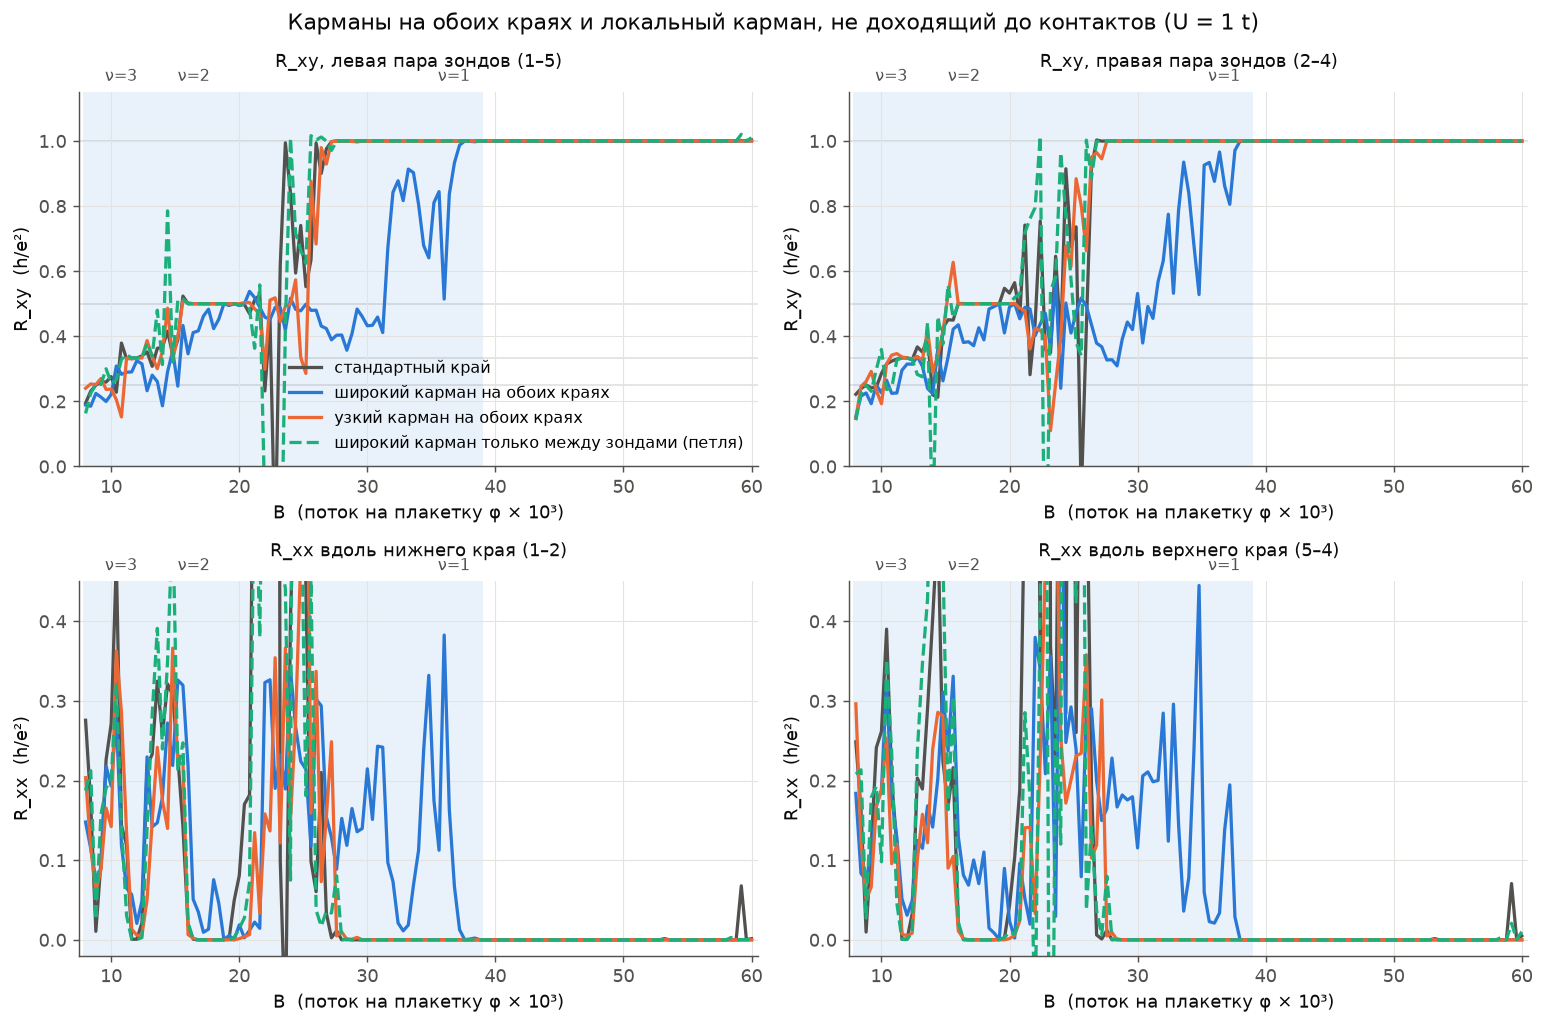
\includegraphics[width=\textwidth]{fig4_both_edges_and_local.png}
\caption{Карманы на обоих краях и локальный карман, не доходящий до
контактов ($U=1\,t$).}
\label{fig:both}
\end{figure}

\subsection{Где течёт ток}
На рис.~\ref{fig:current}~--- плотность тока электронов, выпущенных зондом 2.
В эталоне весь ток идёт по киральному пути $2\to1$. В широком кармане без
беспорядка виден второй путь: встречный канал уносит часть потока из зонда 2
вправо, к стоку 3, т.\,е. против киральности. С беспорядком этот путь
ослаблен, но сохраняется. В узком кармане с беспорядком остаются только
локализованные кольцевые токи вокруг резонансов беспорядка, и встречный путь
к стоку 3 не доходит.

\begin{figure}[ht]
\centering
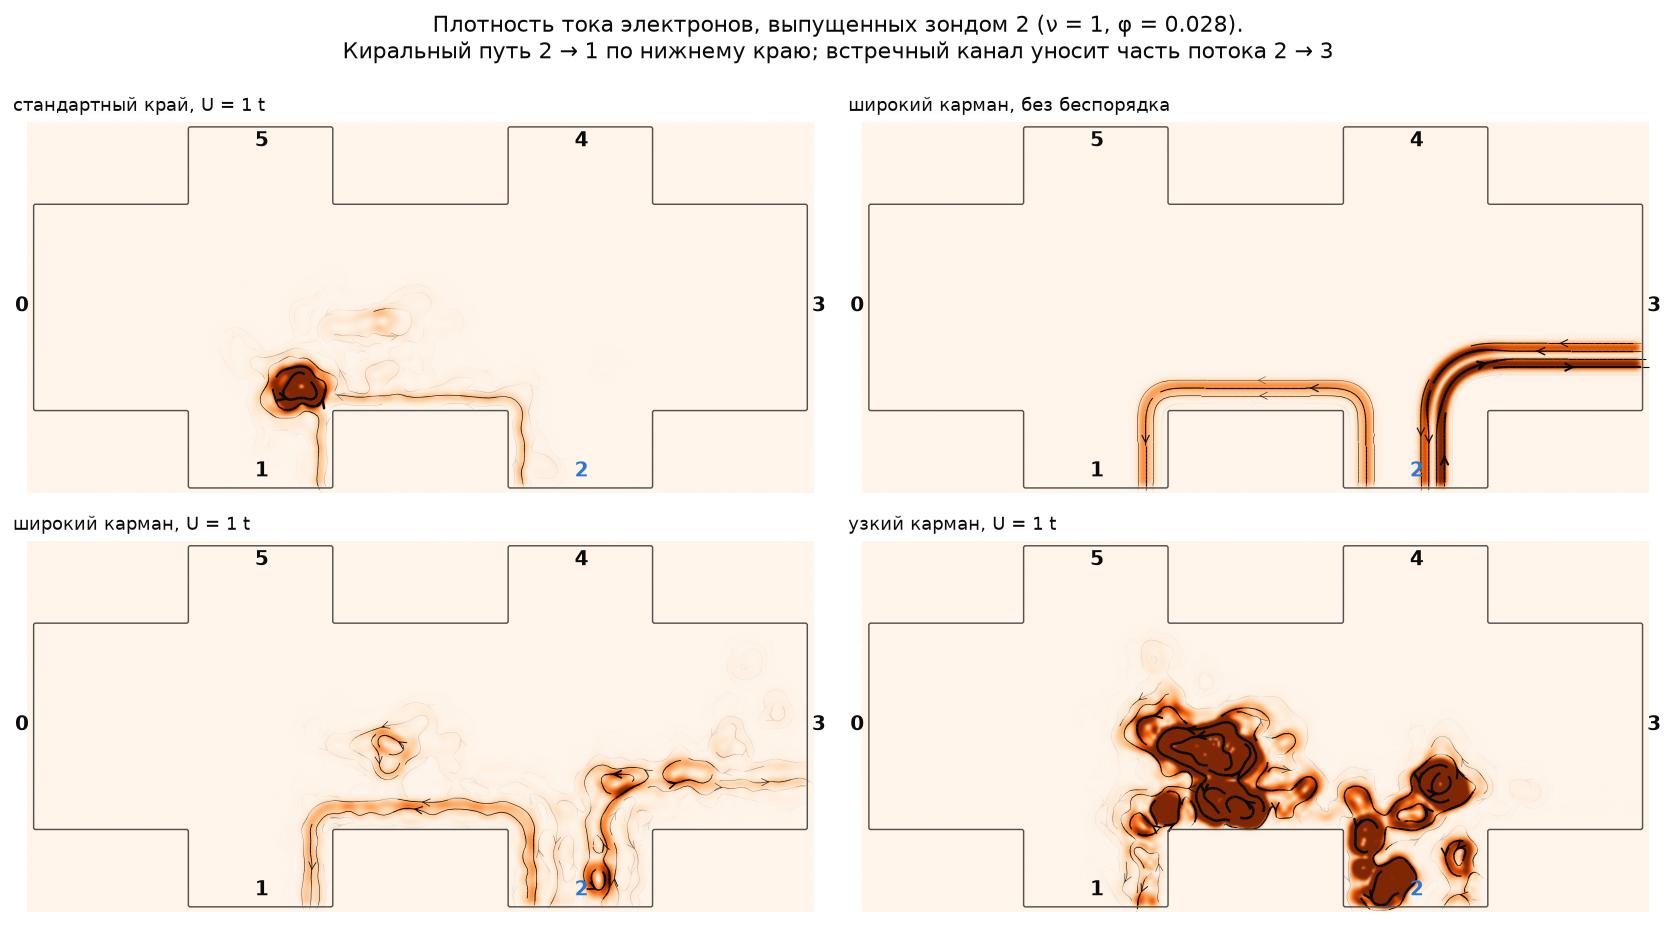
\includegraphics[width=\textwidth]{fig7_injection_from_probe2.png}
\caption{Плотность тока электронов, выпущенных зондом 2 ($\nu=1$,
$\varphi=0.028$). Цветовая шкала общая и обрезана сверху.}
\label{fig:current}
\end{figure}

%======================================================================
\section{Потенциал изображения из~\cite{andolina}}\label{sec:image}

\subsection{Что утверждает работа~\cite{andolina}}
Одноэлектронная модель: $U_\text{im}=-e^2/(8\pi\varepsilon|x-d_\text{edge}|)$
плюс крутой удерживающий потенциал дают яму у края. Масштаб энергии~---
\emph{энергия обратного рассеяния}
\begin{equation}
\Gamma_\ell=\lB\sqrt{\ell+1}\;\partial_xU_\text{im}\big|_\text{край}
=\frac{e^2}{8\pi\varepsilon}\frac{\lB\sqrt{\ell+1}}{d_\text{edge}^2},
\end{equation}
перепад потенциала на размере орбиты. Когда $\EF$ отстоит от дна кармана не
больше чем на $\sim\Gamma_\ell$, встречные состояния находятся на расстоянии
$\lesssim\lB\sqrt{\ell+1}$, электроны рассеиваются назад, и двухтерминальный
$G(\EF)$ не квантован. Расчёты Kwant в~\cite{andolina} (модель
Харпера--Хофштадтера, подводы без поля) дают только двухтерминальный
кондактанс; наиболее хрупкими оказываются зеемановские (нечётные) плато.

\subsection{Параметры}
Используем профиль~\eqref{eq:img}: $d_\text{edge}=18\,a\approx8\,\lB$ при
$\nu=1$ (то же отношение $d_\text{edge}/\lB$, что в оценке~\cite{andolina}
для эксперимента), $E_\text{img}=9$. Тогда глубина ямы
$0.22\,t\approx0.58\,\hw$ и $\Gamma_0=0.036\,t\approx0.1\,\hw$ при
$\varphi=0.03$~--- между «реалистичной» оценкой~\cite{andolina}
($\Gamma_0/\hw\sim0.02$) и значениями $0.2$--$0.4$ на рисунках этой работы.
Карман только на нижнем крае, включая нижние зонды и подводы.

В таком кармане разнесение пары не задано шириной окна, а растёт с энергией
(рис.~\ref{fig:imgprof}, справа): у дна кармана партнёры перекрываются
($O>0.3$ в окне $\approx\Gamma_0$ над дном), выше расходятся до
10--15~$\lB$. Поэтому в одном кармане есть оба режима раздела~\ref{sec:rect}
при разных $\EF$ или $B$. Кроме того, внутренний партнёр лежит на пологом хвосте
$1/d$, и его скорость в 4--5 раз меньше, чем в прямоугольном кармане
($v\approx0.04$--$0.05$ против $0.16$--$0.21$ в единицах $ta/\hbar$), так что
беспорядок рассеивает его назад и при заметном разнесении пары.

\begin{figure}[ht]
\centering
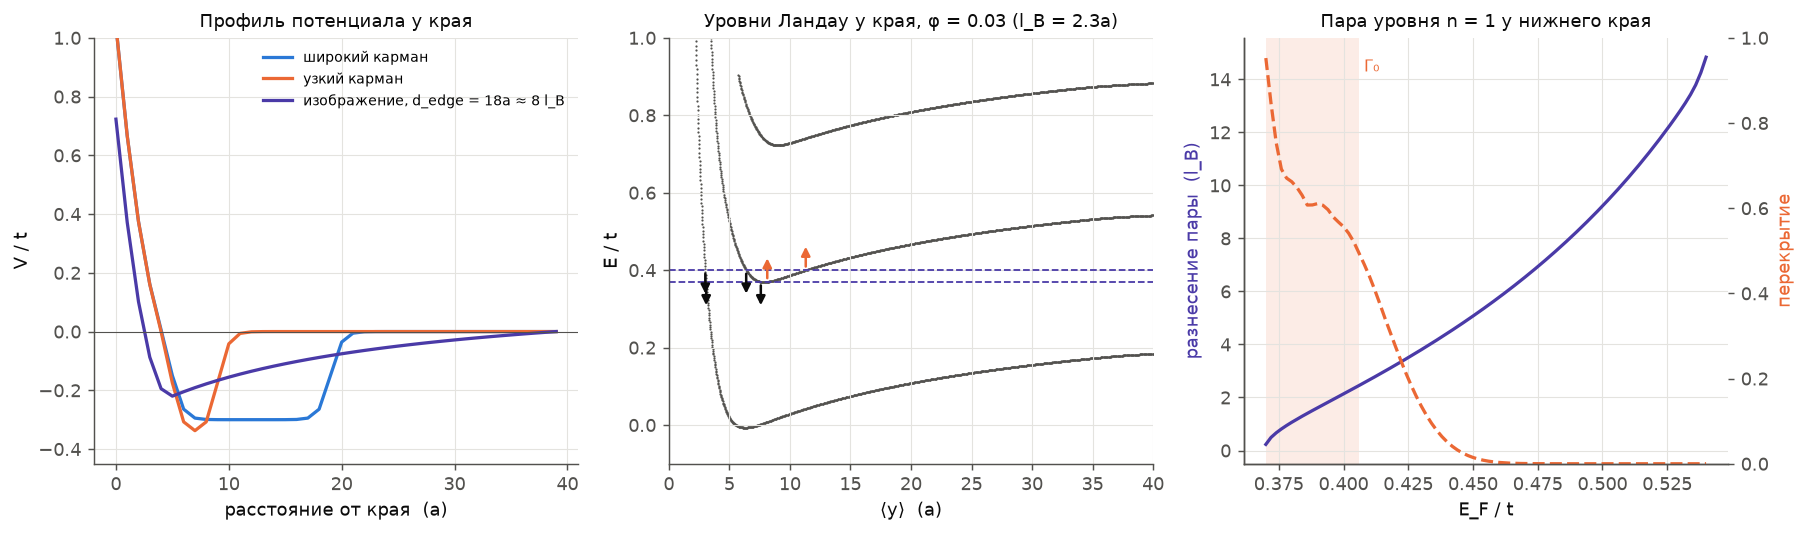
\includegraphics[width=\textwidth]{fig8_image_profile.png}
\caption{Слева: профили края (широкий, узкий карманы и потенциал
изображения). В центре: изогнутые уровни Ландау у края с потенциалом
изображения при $\varphi=0.03$ и моды на двух энергиях Ферми. Справа:
разнесение пары уровня $n=1$ и перекрытие в зависимости от $\EF$; заливка~---
окно $\Gamma_0$ над дном кармана.}
\label{fig:imgprof}
\end{figure}

\subsection{Развёртка по полю}
При $\EF=0.4\,t$ (рис.~\ref{fig:imgB}):
\begin{itemize}
\item Без беспорядка~--- снова точно табл.~\ref{tab:lb} с $\tb=1$ во всём
  окне, где есть пара: при $\nu=1$ $\Rxy^{(1\text{--}5)}=1/2$,
  $\Rxy^{(2\text{--}4)}=3/4$, $\Rxx^\text{низ}=1/4$; при $\nu=2$ и 3~---
  $1/3,\,4/9,\,1/9$ и $1/4,\,5/16,\,1/16$. Заметим, что
  $\Rxy^{(1\text{--}5)}=1/(\nu+1)$ выглядит как продолжение соседнего плато;
  пару выдают только $\Rxy^{(2\text{--}4)}$ и $\Rxx$ нижнего края.
\item С беспорядком на высокополевой части окна ($\varphi\approx0.029$--$0.032$,
  пара перекрыта) $\tb\le0.11$ (среднее по сегментам) и
  $\Rxy^{(1\text{--}5)}=0.86$--$1.00$. На низкополевой части (пара разнесена)
  $\Rxy^{(1\text{--}5)}$ опускается до 0.44--0.70, а $\Rxx^\text{низ}$
  поднимается до 0.33. Это окно, однако, совпадает с объёмным переходом
  $2\to1$ эталона, поэтому ниже то же сравнивается при фиксированном поле.
\end{itemize}

\begin{figure}[ht]
\centering
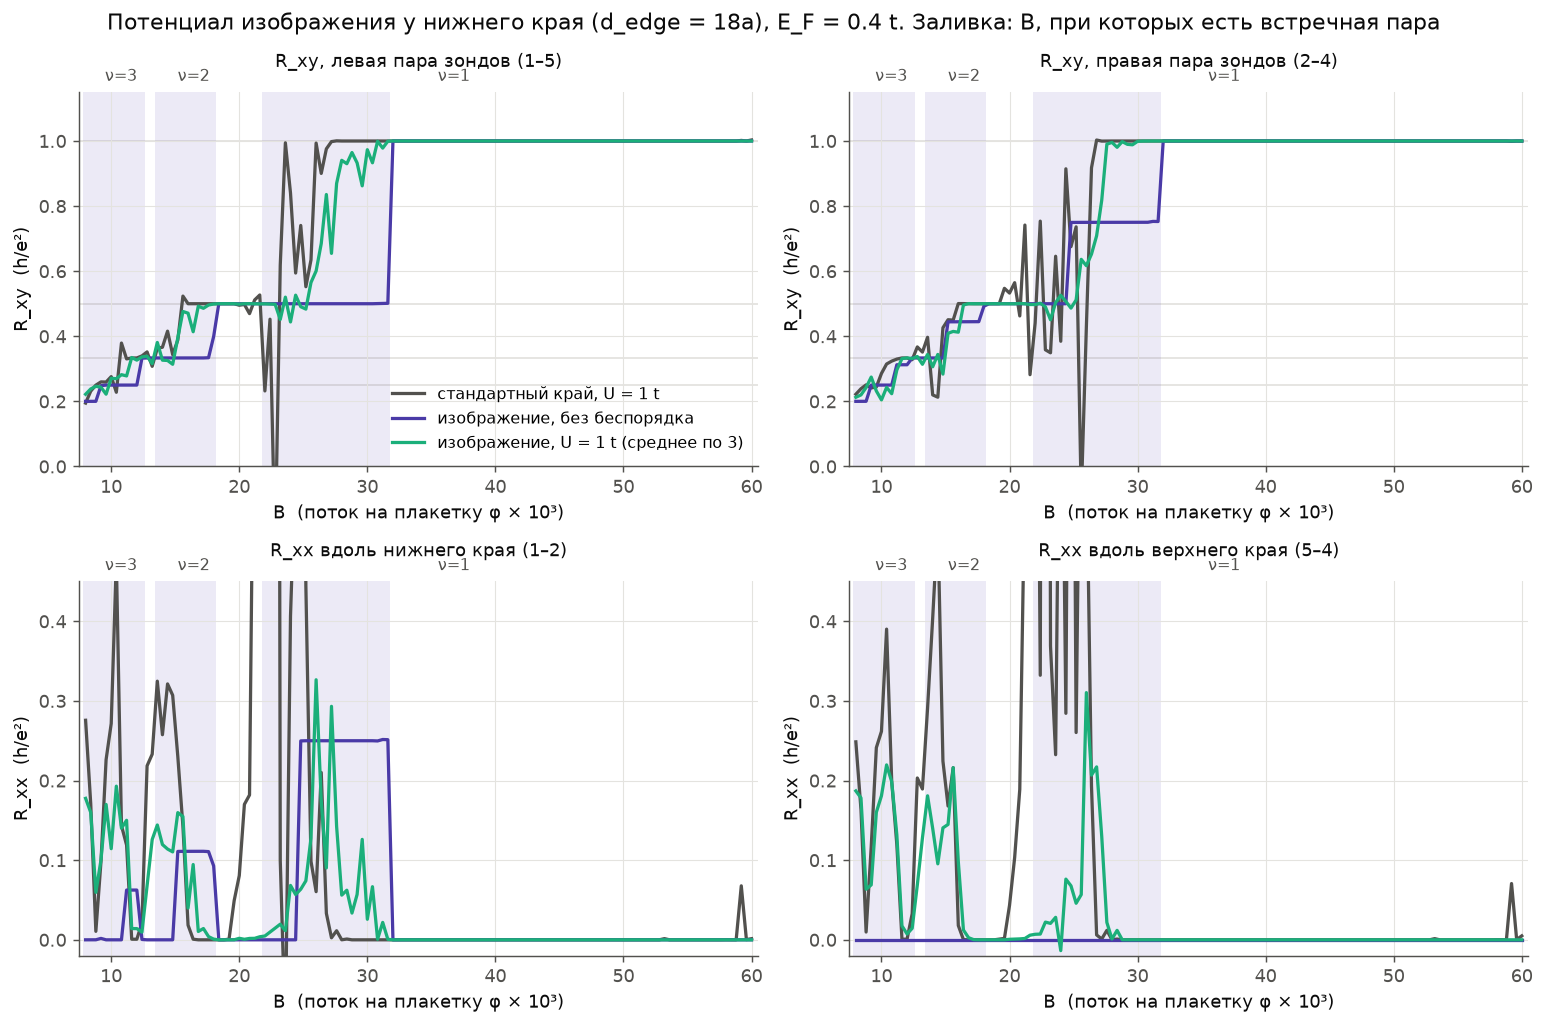
\includegraphics[width=\textwidth]{fig9_image_B_sweep.png}
\caption{Потенциал изображения у нижнего края, развёртка по полю при
$\EF=0.4\,t$. Заливка~--- поля, при которых есть встречная пара.}
\label{fig:imgB}
\end{figure}

\subsection{Развёртка по $\EF$ при фиксированном поле (протокол~\cite{andolina})}
При $\varphi=0.03$ один и тот же образец посчитан и как холловский мостик, и
как простой двухтерминальный брусок (рис.~\ref{fig:imgEF},
табл.~\ref{tab:ef}). Значения с беспорядком усреднены по трём реализациям.

\begin{table}[ht]
\centering
\caption{Развёртка по $\EF$ при $\varphi=0.03$, потенциал изображения,
$U=1\,t$. При $\EF<0.19$ объём пуст, у верхних зондов нет каналов, и мостик
не измерить; остаётся только $G_\text{2t}$.}
\label{tab:ef}
\resizebox{\textwidth}{!}{%
\begin{tabular}{@{}lllccc@{}}
\toprule
$\EF/t$ & пара & $G_\text{2t}$, $e^2/h$ & $\Rxy^{(1\text{--}5)}$ & $\Rxx^\text{низ}$ & эталон $\Rxy$, $\Rxx$\\
\midrule
0.000--0.048 ($\nu=0$) & 0.8--3.2 $\lB$ & $\le0.003$ (без беспор.\ 1) & --- & --- & $G_\text{2t}=0$\\
0.052--0.12 ($\nu=0$) & 3.4--7.9 $\lB$ & $0.07\to0.98$ & --- & --- & $G_\text{2t}=0$\\
0.372--0.412 ($\nu=1$) & 0.5--2.8 $\lB$, $O$=0.85--0.41 & 1.000 & 0.97--1.00$^a$ & $\le0.03^a$ & 1, 0\\
0.416--0.432 ($\nu=1$) & 3.0--3.9 $\lB$, $O$=0.34--0.11 & 0.986--1.000 & 0.81--0.91 & 0.09--0.19 & 1, $\le10^{-4}$\\
0.436--0.448 ($\nu=1$) & 4.2--4.9 $\lB$, $O\le0.08$ & 0.89--1.035 & 0.73--0.92 & 0.09--0.29 & 1, $\le0.016$\\
0.372--0.49, $U=0$ & & 2 & 0.50 & 0.25 & \\
\bottomrule
\end{tabular}}\\[2pt]
{\footnotesize $^a$ одна точка: $\Rxy=0.88$, $\Rxx=0.12$.}
\end{table}

\begin{itemize}
\item \textbf{Окно $\nu=0$~--- аналог рисунков~3 и S1 из~\cite{andolina}.}
  Над дном кармана $G_\text{2t}<1$ и растёт к 1 по мере расхождения пары. В
  нашем длинном образце с сильным беспорядком это окно шире $\Gamma_0$, и
  внутри него $G_\text{2t}=0$ (встречный канал локализован целиком), а не
  частично подавлен.
\item \textbf{Окно $\nu=1$~--- главное различие двух измерений.} Пока пара
  перекрыта, она локализована, и квантованы оба измерения. Когда партнёры
  расходятся на 3--4~$\lB$, мостик уже заметно не квантован
  ($\Rxx^\text{низ}=0.09$--$0.19$, эталон квантован до $10^{-4}$), а
  $G_\text{2t}$ всё ещё равен 0.986--1.000. В отдельных реализациях
  $\Rxx^\text{низ}$ доходит до 0.4, а $\tb$ отдельных сегментов~--- до 0.55.
\item С $\EF\approx0.436$ эталон начинает отклоняться от квантования, а при
  $\EF\ge0.452$ у него начинается объёмный переход, и сравнение теряет смысл.
\end{itemize}

\begin{figure}[ht]
\centering
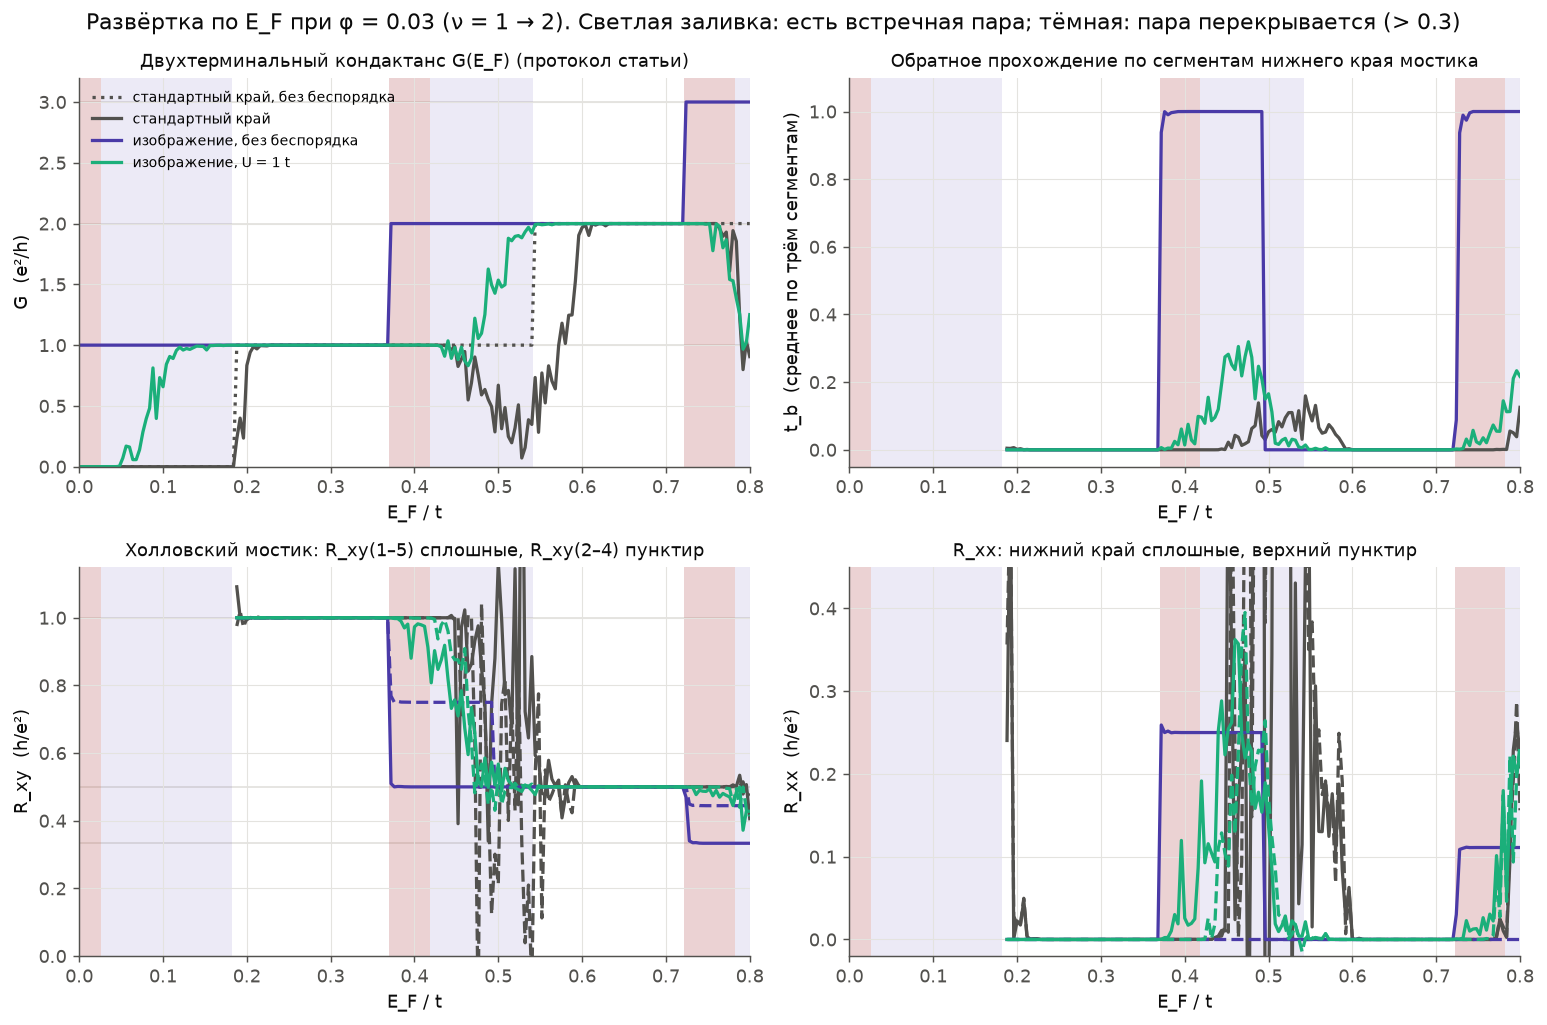
\includegraphics[width=\textwidth]{fig10_image_EF_sweep.png}
\caption{Развёртка по $\EF$ при $\varphi=0.03$. Светлая заливка~--- есть
встречная пара, тёмная~--- пара перекрыта ($O>0.3$). Сверху слева:
двухтерминальный кондактанс бруска (протокол~\cite{andolina}); сверху справа:
$\tb$, усреднённое по трём сегментам нижнего края мостика; снизу:
сопротивления мостика.}
\label{fig:imgEF}
\end{figure}

%======================================================================
\section{Интерпретация и сравнение с~\cite{andolina,ciuti}}

\begin{enumerate}
\item \textbf{Одна физика, разные наблюдаемые.} По~\eqref{eq:g2t}
  двухтерминальный кондактанс целый и при $\tb=0$ (пары как будто нет), и
  при $\tb=1$ (баллистическая пара считается ещё одним каналом); виден только
  промежуточный $\tb$. В мостике $\tb$ каждого сегмента между соседними
  контактами даёт $\Rxx$ и разницу холловских напряжений, а $\tb=1$
  даёт \emph{максимальное} отклонение. «Нарушение квантования»
  в~\cite{andolina} (промежуточный $\tb$ у дна кармана) и «защита квантования
  обратным рассеянием» из раздела~\ref{sec:rect}~--- два конца одной
  зависимости $\tb$ от разнесения пары. Что наблюдается, зависит от длины
  края между контактами, силы беспорядка и способа измерения.
\item \textbf{Метки плато разные.} В~\cite{andolina} «квантовано»~--- это
  $G=\nu+1$ над дном кармана (баллистическая пара сосчитана как канал), а
  нарушение~--- $G<\nu+1$ в окне $\Gamma_\ell$. Для мостика с объёмным
  заполнением $\nu$ квантование означает $\Rxy=h/\nu e^2$ и $\Rxx=0$, т.\,е.
  $\tb=0$.
\item \textbf{Четырёхтерминальное измерение чувствительнее.} Сегмент между
  зондами (60--70~$a$) короче всего края (300~$a$), и $\tb\sim e^{-L/\xi}$ на
  нём больше. При $\EF=0.416$--$0.432$ $G_\text{2t}$ отличается от 1 не
  больше чем на 0.015, а $\Rxx^\text{низ}$ того же образца~--- 0.09--0.19~$\he$.
\item \textbf{Комментарий~\cite{ciuti}.} Первое возражение (кармана нет
  из-за донорного фона, пиннинга уровня Ферми на протравленной поверхности и
  ёмкости поверхностных состояний $\gg\varepsilon_0/d$) мы не проверяем: все
  выводы условны~--- \emph{если} карман есть. На второе (статья не считает
  $\Rxx$ и $\Rxy$) наш расчёт отвечает прямо: в шеститерминальном мостике
  такой карман даёт $\Rxx\neq0$ \emph{только вдоль края рядом с металлом},
  разные $\Rxy$ на двух парах зондов (разница равна $\Rxx$ этого края) и
  отклонения только на низкополевой стороне плато. Это отличает механизм от
  объёмного (например, вакуумного), при котором $\Rxx$ появляется вдоль обоих
  краёв.
\item \textbf{Чего здесь нет из~\cite{andolina}:} спина и зеемановских
  плато, конечной температуры, работы при фиксированном числе частиц.
  Подводы в коде~\cite{andolina} без поля и без кармана, у нас~--- с полем и
  карманом; в обоих случаях встречный канал заканчивается в контакте, так что
  на вывод это не влияет.
\end{enumerate}

%======================================================================
\section{Выводы и экспериментальные признаки}

\begin{enumerate}
\item Встречный партнёр кирального канала появляется, если у края есть
  карман глубиной порядка расстояния от $\EF$ до следующего уровня Ландау.
  Это происходит на низкополевой стороне каждого плато.
\item Интуиция «обратное рассеяние на одном краю не должно портить холловский
  отклик» верна, причём в более сильной форме: обратное рассеяние внутри края
  не может нарушить квантование, оно его защищает. Всё, что происходит внутри
  края между двумя контактами, сводится к $\tb$, а квантование нарушается
  только при $\tb\neq0$.
\item Отклонения $\Rxy$ от $h/\nu e^2$ и $\Rxx\neq0$ появляются, когда
  встречный канал \emph{не} рассеивается назад (партнёры не перекрываются)
  \emph{и} доходит до омических контактов. Объёмная $\sigma_{xy}$ при этом
  остаётся $\nu e^2/h$~--- это эффект контактов и геометрии, а не разрушение
  топологии.
\item С потенциалом изображения из~\cite{andolina} картина та же. Когда
  партнёры расходятся, $\Rxx$ и разница холловских напряжений появляются в
  мостике раньше, чем отклонение двухтерминального $G$.
\end{enumerate}
Признаки сценария в эксперименте:
\begin{itemize}
\item $\Rxx\neq0$ только вдоль края, рядом с которым есть карман (металл);
\item холловские напряжения на разных парах зондов различаются ровно на
  $\Rxx$ этого края;
\item эффект сосредоточен на низкополевой стороне плато и исчезает, если
  карман не доходит до контактов;
\item двухтерминальное измерение может его почти не показывать.
\end{itemize}

%======================================================================
\section{Ограничения}
\begin{itemize}
\item Модель одночастичная и когерентная: нет электрон-электронного
  взаимодействия, реконструкции края и неупругой эквилибрации между каналами.
  Эквилибрация на длинах, больших длины эквилибрации, тоже даёт $\tb\to0$
  (как для $\nu=2/3$).
\item Карман задан руками; вопрос о том, возникает ли он в самосогласованной
  электростатике реальной мезы~\cite{ciuti,chklovskii}, здесь не решается.
\item Образец мезоскопический ($L\approx125\,\lB$), поэтому переходы между
  плато сильно флуктуируют. Основные кривые усреднены по трём реализациям
  беспорядка, часть кривых~--- одна реализация.
\item Параметры карманов выбраны для наглядности, а не подогнаны под
  конкретный эксперимент.
\end{itemize}

%======================================================================
\appendix
\section{Воспроизводимость}
Код и данные~--- каталог \texttt{qhe\_pockets/} репозитория:
\texttt{model.py} (геометрия, потенциалы, транспорт), \texttt{lb.py}
(модель Ландауэра--Бюттикера), \texttt{edge\_modes.py} (моды ленты),
\texttt{run\_sweeps.py}, \texttt{width\_sweep.py}, \texttt{image\_sweeps.py}
(расчёты), \texttt{plots.py}, \texttt{plots\_image.py} (рисунки).
\begin{verbatim}
conda install -c conda-forge kwant matplotlib scipy
OMP_NUM_THREADS=1 python run_sweeps.py    # ~1 ч на 4 ядрах
OMP_NUM_THREADS=1 python width_sweep.py   # ~20 мин
OMP_NUM_THREADS=1 python image_sweeps.py  # ~20 мин
python plots.py && python plots_image.py
\end{verbatim}
Замечание о калибровке: \texttt{kwant.physics.magnetic\_gauge} требует
$B=2\varphi$, чтобы получить $\varphi$ квантов потока на плакетку (проверено
для Kwant 1.5).

\begin{thebibliography}{9}
\bibitem{andolina} G.~M.~Andolina, Z.~Bacciconi, A.~Nardin, M.~Schirò,
  P.~Rabl, D.~De~Bernardis, \emph{Electrostatics-induced breakdown of the
  integer quantum Hall effect in cavity QED},
  \href{https://arxiv.org/abs/2511.04744}{arXiv:2511.04744}.
\bibitem{ciuti} C.~Ciuti, G.~Scalari, J.~Faist, \emph{Comment on
  ``Electrostatics-induced breakdown of the integer quantum Hall effect in
  cavity QED''}, \href{https://arxiv.org/abs/2601.14974}{arXiv:2601.14974}.
\bibitem{appugliese} F.~Appugliese \emph{et al.}, \emph{Breakdown of
  topological protection by cavity vacuum fields in the integer quantum Hall
  effect}, Science \textbf{375}, 1030 (2022).
\bibitem{buttiker} M.~Büttiker, \emph{Absence of backscattering in the
  quantum Hall effect in multiprobe conductors}, Phys.\ Rev.\ B \textbf{38},
  9375 (1988).
\bibitem{kwant} C.~W.~Groth, M.~Wimmer, A.~R.~Akhmerov, X.~Waintal,
  \emph{Kwant: a software package for quantum transport}, New J.\ Phys.\
  \textbf{16}, 063065 (2014).
\bibitem{chklovskii} D.~B.~Chklovskii, B.~I.~Shklovskii, L.~I.~Glazman,
  \emph{Electrostatics of edge channels}, Phys.\ Rev.\ B \textbf{46}, 4026
  (1992).
\end{thebibliography}

\end{document}
